\documentclass{article}

\usepackage{amsthm}
\usepackage{amsmath}
\usepackage{amssymb}
\usepackage{graphicx}

\title{CS3410 Project 1 Design Document}
\date{February 25, 2015}
\author{Alexandra Anderson, Joshua Hull}

\begin{document}
\maketitle

\section*{Introduction}
Our MIPS processor will follow a five stage pipeline as discussed in class.  Each stage will be blocked off with registers storing necessary data.  Instructions will proceed through one stage of the pipeline per clock cycle. The overall diagram of how the stages are laid out is as follows:

\begin{figure}[h]
	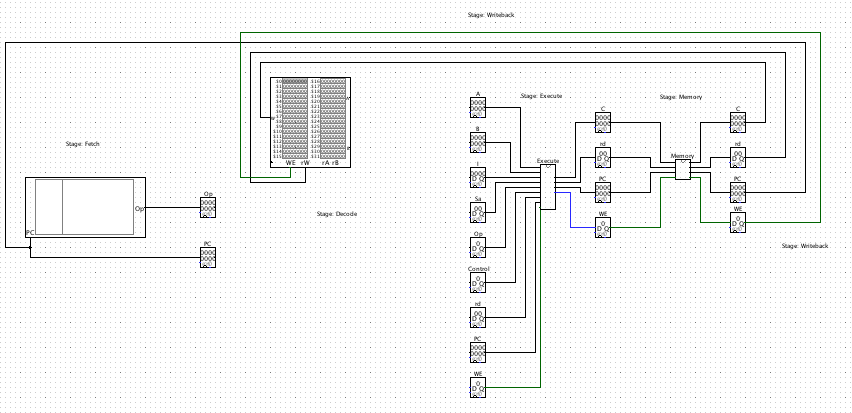
\includegraphics[width = \textwidth]{layout}
	\caption{The layout of the MIPS pipeline in five stages.}
\end{figure}

This is merely a design diagram. While we will implement the pipeline processor in the overall layout and sub circuits shown, very few wires are currently connected. The fetch, decode, and execute stages are not yet implemented, although space for them has been allocated. 

\section*{Fetch}
This stage Fetches the next instruction from the instruction memory and updates the program counter.  Both the instruction and PC$+4$ are passed into the register so that the next stage (Decode) has access to that information.  

To calculate PC$+4$, we split off the lower two digits of the PC, use the $+1$ incremented to increment the remaining 30 bits, and rejoin them into one 32 bit bus. 

The Fetch stage will also include a multiplexer to select between PC$+4$ and jump/branch targets, for Project 2. 

\section*{Decode}
This stage uses the bits in the instruction to determine several different values:

It determines the immediate value for immediate operations (this value is computed regardless of whether or not the operation is an immediate operation - it is selected for using a multiplexer in the next stage).

It determines which registers to read from (and reads those registers).

It determines a shift amount and op-code to send to the ALU.

It also determines jump and branch amounts (though these values are not used).

The registers at the end of this stage will store certain data for the next stage including the values of the read registers, PC$+4$, jump and branch targets, the immediate value, the shift amount, the op code, the write enable bit, and the register to write to. There are also two extra control bits indicating the presence of a set less than operation and whether it is signed or unsigned, one more indicating whether this is an immediate or register operation, and two dealing with the three conditional move or load operations. 

We include a simplified truth table to show how the decoding logic will work. Op[6] refers to the op-code, the first 6 bits of the operation. Func[6] refers to the final 6 bits of the operation. The ALU[4] is the 4-bit control signal passed directly into the ALU. 

\begin{tabular}{| c | c  c  c  c  c  c | c c c c c c | c c c c |}
\hline
OPCODE & OP[6] &&&&&& FUNC[6] &&&&&& ALU[4] &&&\\
\hline
ADDI	&0	&0	&1	&0	&0	&1	&x	&x	&x	&x	&x	&x	&0	&0	&1	&x \\
ANDI	&0	&0	&1	&1	&0	&0	&x	&x	&x	&x	&x	&x	&1	&0	&0	&0 \\
ORI		&0	&0	&1	&1	&0	&1	&x	&x	&x	&x	&x	&x	&1	&0	&1	&0 \\
XORI	&0	&0	&1	&1	&1	&0	&x	&x	&x	&x	&x	&x	&1	&1	&0	&0 \\
SLTI		&0	&0	&1	&0	&1	&0	&x	&x	&x	&x	&x	&x	&x	&x	&x	&x \\
SLTIU	&0	&0	&1	&0	&1	&1	&x	&x	&x	&x	&x	&x	&x	&x	&x	&x\\
\hline
ADDU	&0	&0	&0	&0	&0	&0	&1	&0	&0	&0	&0	&1	&0	&0	&1	&x\\
SUBU	&0	&0	&0	&0	&0	&0	&1	&0	&0	&0	&1	&1	&0	&1	&1	&x\\
AND		&0	&0	&0	&0	&0	&0	&1	&0	&0	&1	&0	&0	&1	&0	&0	&0\\
OR		&0	&0	&0	&0	&0	&0	&1	&0	&0	&1	&0	&1	&1	&0	&1	&0\\
XOR		&0	&0	&0	&0	&0	&0	&1	&0	&0	&1	&1	&0	&1	&1	&0	&0\\
NOR		&0	&0	&0	&0	&0	&0	&1	&0	&0	&1	&1	&1	&1	&1	&1	&0\\
\hline
\end{tabular}

This represents a limited subset of the supported operations, and a limited subset of control bits. 

\section*{Execute}
This section sign-extends the immediate value and selects whether to use register B or the immediate value in the operation.  Then, it performs the given ALU operation.

This result is then combined with some additional logic (comparators in the case of SLT  or MOVZ for instance) and the result of the operation is outputted.

\begin{figure}[h]
	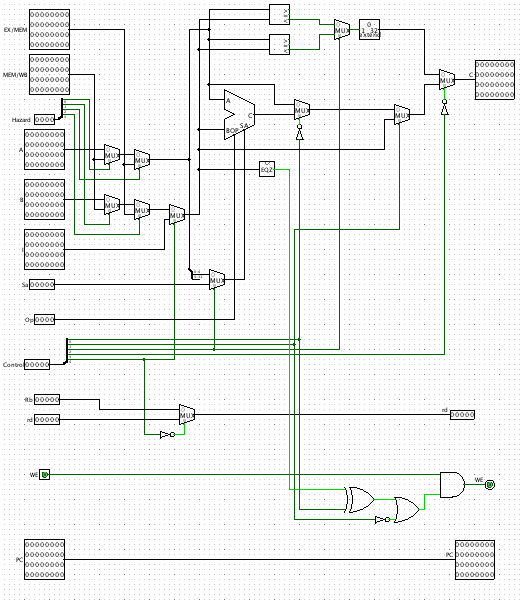
\includegraphics[width = \textwidth]{execute}
	\caption{The Execute pipeline stage}
\end{figure}

The execute circuit has hazard detection in the top left, arithmetic computation and control in the top right, and write enable and target register computations at the bottom. Moving is conditional, so we compute the conditions and the controls that say whether we're moving into the write enable. The destination register is stored in a different part of the original operation for immediate arithmetic. 

We implement data hazard detection using forwarding, with a dedicated hazard detection sub circuit. There will be no control or memory hazards in Project 1, because we do not support branching, jumping, or memory operations. Therefore, the correct data will be stored in pipeline registers farther ahead, and we can easily use forwarding to resolve all hazards. 

The registers at the end of this stage will store PC$+4$, the result of the ALU operation, the write enable bit, and the register to write to.

\section*{Memory}
This section will be a pass-through stage. There will not be any logic here, though it will be blocked off by registers so all operations have to spend a cycle in this stage. The registers at the end of this stage store the same values as the registers at it's beginning, for Project 1. 

\section*{Writeback}
This section will only write the results of the register and immediate operations that we have to implement.  It will not write the bits read from memory (as these operations will not be implemented).

\end{document}